\documentclass[a4paper,11pt]{article}

\usepackage[latin1]{inputenc}
\usepackage[T1]{fontenc}
\usepackage{bbm} %math chars
\usepackage{amsmath}
\usepackage{indentfirst}
\usepackage{fullpage} %minimizes the default margins
\usepackage{url}
\usepackage{graphicx}
\usepackage[center,footnotesize]{caption} %options des legendes des graphes
\usepackage[section]{placeins} %place les figures d'une section avant le debut de la suivante
\usepackage{subfig} %a) b) c)
\usepackage{fancyvrb}
\usepackage{color}
\usepackage{url}
\usepackage[colorlinks=true,linkcolor=black,citecolor=black,urlcolor=blue]{hyperref}
\usepackage{fancyvrb}

\begin{document}
\title{Exercises - Week 13}
\date{}
\author{Genomics and bioinformatics}
\maketitle

\section{Motif model}

\noindent Suppose we are given the following four aligned binding sites of a particular TF:

\begin{figure}[h!]
\centering
\begin{BVerbatim}
TTGACT
TCGATA
TTGAAA
TCGAGT
\end{BVerbatim}
\hspace{15mm}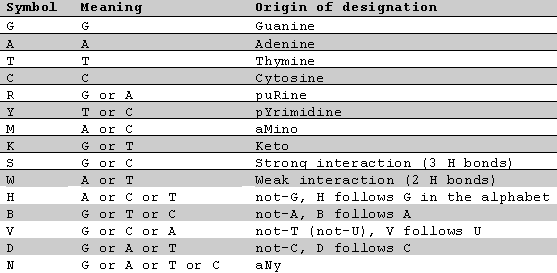
\includegraphics[width=11cm]{IUPAC.png}
\caption{The DNA binding site sequences and the IUPAC-IUB code.}
\end{figure}

\noindent These sequences share some common pattern that can be represented by the consensus sequence or the Positional Weight Matrix (PWM) and its logo. The consensus sequence represents each position by the most frequent base; if an equal number of different bases are present, the position is represented by a set of those bases. Note that for short-hand notation the set is represented by the IUPAC-IUB code (see Figure~1).  The matrix elements $M_{ij} = \exp(W_{ij})$, where $W$ is the PWM introduced in the lectures, represent each position by the frequency of the 4 bases in the aligned binding sites. More precisely, the matrix $M$ is a $4 \times L$ matrix, where the $4$ rows corresponds to the letters A, C, G and T, and the $L$ columns corresponds to the length of the sequences (here $L=6$). Note that $\sum_{i \in \{A, C, G, T\}} M_{ij} = 1$, $\forall j$. The matrix M can be visualised graphically using a logo: the information content at position $j$ is
$$
I_j = 2 + \sum_{i \in \{A, C, G, T\}} M_{ij} \cdot \log_2(M_{ij}) \in [0,2] ~.
$$
Here we assume that $M_{ij} \cdot \log_2(M_{ij})=0$ if $M_{ij}=0$. Note by comparing with the lecture notes that we have set for simplicity $f_i = 1/4$ for the background frequencies. The height of the character $i$ at position $j$ is given by 
$$
\mbox{Height}_{ij} = M_{ij} \cdot I_j~.
$$
\noindent \textit{Question:} Write the consensus sequence, compute the matrix $M$ and draw a sketch of its logo for the four binding site sequences given in the above figure.\\

\noindent \textit{Indication:} Use the relation $\log_2(2^{-k})=-k$.

\newpage
\section{Motif finding}

\noindent Suppose a ChIP-seq experiment with an anti-body specific to some TF has been realised. After peak calling, we obtain a set of DNA sequences that are possibly bound by the same TF:

\begin{figure}[h!]
\centering
\begin{BVerbatim}
ATTGACAC
CCTTGACA
TTGACA
ATTGACAC
\end{BVerbatim}
\end{figure}

\noindent The aim of motif finding is to search for the common binding pattern and represent it by the consensus sequence or the matrix $M$. Here we are going to search for a motif of length $L=6$: we break the four above binding site sequences into all possible length $L$ substrings $\{S_1, \dots, S_N\}$, where $N=10$. The likelihood of observing the provided $N$ sequences for a given matrix $M$ is
$$
\mathcal{L}(M) = P(S_1,\dots,S_N | M) = \prod_{k=1}^N  P(S_k | M) = \prod_{k=1}^N \prod_{j=1}^L M_{S_{kj},j}~.
$$
We want to find the matrix $M^*$ having the largest likelihood:
$$
M^* = \mbox{argmax}_{M} \{\mathcal{L}(M)\}~.
$$
Starting with an initial $M$, we shall use the Expectation-Maximization (EM) algorithm to find a local optimum of $\mathcal{L}(M)$. \\

\noindent Proceed as follows:

\begin{enumerate}
\item Break the four above binding sites into the $N=10$ possible substrings of length $L=6$.
\item Considering these $N=10$ sequences together (similarly to the 4 sequences in Exercise 1), compute the initial matrix $M$.
\item Apply the Expectation step: for every sequence $S_k$ compute the probability that $S_k$ is a motif:
$$
p_k = P(S_k | M) = \prod_{j=1}^L M_{S_{kj},j}~.
$$
\item Apply the Maximization step: compute the updated $M$ by 
$$
M_{ij} = \frac{1}{\sum_{k=1}^N p_k} \cdot \sum_{\substack{\ell = 1 \\ S_{\ell j} = i }}^N p_\ell~.
$$
In principle, one should repeat the expectation and maximization steps several times to reach a local optimum of $\mathcal{L}(M)$. Note that in general this local optimum depends strongly on the initial matrix $M$.
\item Compare the consensus sequences associated to the initial and updated matrices $M$. Looking back at the four binding site sequences, was it expected ?
\end{enumerate}

\end{document}
